\section{Methods}
\label{sec:methods}
\begin{figure}[tb]
  \begin{center}
    \begin{tabular}{ccc}
    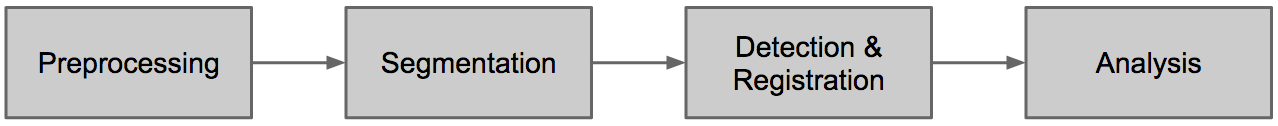
\includegraphics[width=\figfullwidth] {fig/framework.png}
    \end{tabular}
    \caption{ \label{fig:framework} Illustration of the proposed 4D CT image processing framework. From CT image preprocessing, image segmentation, landmark detection and functional data registration, to final analysis.
    }
  \end{center}
\end{figure}

% How do I approach it?
In terms of analysis subjects with huge varieties, including age, weight, and length of airway, data registration is an important issue.
To compare different subjects in one metrics, registration between different subjects for compensating the deformation is needed for atlas building.
Along with inter-subject registration, intra-subject registration to different scans in a period of time in critical.
Registration within a subject in a short period of time would be much tractable for registration among different subjects.
Several registration techniques have been developed in different perspectives.
First, registration on image, which uses image intensity as a major feature, has being developed in medical image analysis for past decade.
Most of these methods have to do with defining an energy function with data term (dissimilarity between source image and target image) and regularization term (atypicality of mapping from source image to target image),
and then develop optimization method to find a best mapping which minimizes such energy.
Hill et al. and Sotiras et al. wrote very educated review articles on general registration methods on image intensity~\cite{hill2001medical,otiras2013deformable}.
For particular application for registration on one subject among a short time period, Guerrero et al. developed a deformable algorithm for dynamic ventilation imaging from 4D CT~\cite{guerrero2006dynamic}.
Besides, registration on shape, which uses geometric cues as major features, has succeeded in many applications in computer vision and computer graphics fields~\cite{belongie2002shape,li2012temporally}.
With the same fashion of energy minimization framework as image registration, these methods rely on shape features, e.g. curvature or level of bending, to define the data term.
However, applying those techniques above for aligning pediatric airway 3D CT scans among different subjects was still a hard problem.
No even mention we have variances within each subject due to 4D CT scans.
Hong et al. proposed a simplified airway model which is much easier to register for further analysis~\cite{hong2014statistical}.
I started this project by extending Hong et al.'s simplified airway model to a 4D CT processing framework.
Figure~\ref{fig:framework} illustrated the automatic 4D CT processing framework.


% Need to familiar with
\subsection{Image preprocessing and segmentation}
\label{sec:image_preprocessing_and_segmentation}
For better adaptive to currently medical image processing libraries, the framework start with transform data from DICOM images to NRRD images.
Then a padding and filtering operator for making the image boundary has the same intensity as air is applied on NRRD images.
With scripts automatically applying preprocessing programs reduced cost of manually operating medical image softwares, such as Slicer or ParaView.

The algorithm segmented the airway from 3D CT image using Otsu's method and two manually chosen seeds that bracket the upper airway.
Otsu's method finding a threshold to separate data into two clusters, so as to try to make each cluster as tight as possible.
This is achieved by maximizing the inter-subject variances and minimizing intra-subject variances in terms of voxel intensity.
In our case for segmenting airway, the two clusters were air and non-air regions.
To remove the air regions that were not in the airway, morphological operator erosion first be applied to remove the actual airway.
This computed a map of outside air regions.
We can apply the map as a filter to remove the air outside the airway to get a clean airway in the subject.
Then, two seeds further help to extract trachea and exclude bronchus in the airway.

With this segmentation, the upper airway can be approximated by statical models, including boundary point distribution models, deformation of atlas models, implicit models, or skeletal models~\cite{pizer2013nested}.
Focus on measuring the size of airway, we used a centerline with cross sections to represent the airway.
The centerline is inferred based on the heat distribution along the airway flow that is solved by a Laplace equation.
Cross sections are cut from segmented airway geometry using planes that are orthogonal to the centerline. 
The area of the cross sections would be the 1D functional data representation of an airway.

\subsection{Landmark detection}
\label{sec:landmark_detection}
\begin{figure}[tb]
  \begin{center}
    \begin{tabular}{ccc}
    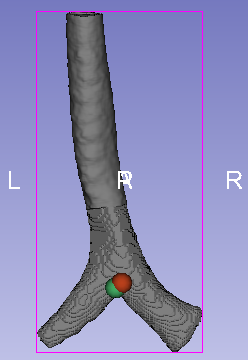
\includegraphics[height=\figheight] {fig/Fleck_005_geometry.png}
    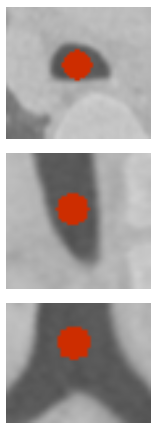
\includegraphics[height=\figheight] {fig/landmark.png}
    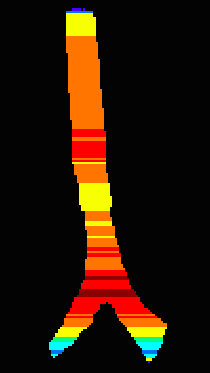
\includegraphics[height=\figheight] {fig/Fleck_005_likelihood.png}
    \end{tabular}
    \caption{ \label{fig:detection} Visualization of the framework of landmark detection. {\bf Left.} First, an airway geometry is segmented by Otsu-thresholding. Green marker is the ground truth annotation and red marker is the predicted location of TC. {\bf Middle.} Second, CHOG features are computed in the center of trachea in each depth. From top to down: Sagittal, coronal, and axial. {\bf Right.} Final, applying the trained classifier on these different hypotheses to get likelihoods of the landmark. Dark red indicates the highest likelihood of TC. In this case, the predicted TC has only 1.97 mm (the total length is 159 mm) away from the ground truth annotation. This error is only 1.2$\%$ of the entire airway.
    }
  \end{center}
\end{figure}

We can register functional data alone with some common landmarks across subjects.
In general, landmark annotation was performed manually.
For reducing the manually annotation cost, based on Dalal and Triggs's object detection framework~\cite{dalal2005histograms}, I propose a landmark detection framework using concatenating Histogram of Gaussian (CHOG) features and geometric prior. Figure~\ref{fig:detection} illustrated a detection of trachea carina (TC).

HOG is well designed normalized local histograms of image gradient orientation in a dense sample grid.
The original purpose of this feature was for human detection.
Given the popularity of HOG based object detectors, researchers even tried to answer why it works (or did not work) by visualizing the feature spaces~\cite{vondrick2013hoggles}.
Nevertheless, HOG captures edge or gradient structure that is very characteristic of local shape in our cases, and it can be efficiently computed.
% what is HOG?
In practice the HOG is implemented by dividing an image window into small spatial cells, for each cell accumulating a histogram of gradient directions with different bins over pixels of the cell.
The concatenated histogram over cells would be the final representation of an image window.

For applying HOG on 3D images, instead of computing histogram over arbitrary 3D orientations, I attempted to computed 2D HOG in axial, coronal, and sagittal plane, which are the three perspectives for user annotations.
This reduced the computational complexity and made learning feasible given limit amount of ground truth images.

The first step of the landmark detection framework then is to train a binary classifier using CHOG.
For doing high dimensional data and low sample size statical analysis, Distance Weighted Discrimination can be applied to improve the training~\cite{marron2007distance}.
Yet, for simplistic and speed, linear Support Vector Machine (SVM) is used as a baseline throughout study.

In prediction stage, the trained classifier can be applied as a filter on hypotheses with different locations and sizes.
Higher score generally implies a higher likelihood of a hypothesis.

After landmarks are located, I registered the functional data to the unified domain~\cite{ramsay2006functional}.
In Hong et al.'s original paper, each subject had five visible landmarks from nasal spine, choana, epiglottis tip, true vocal cord (TVC), and TC.
In our dynamic data, most of subjects only have TVC and TC.
Even thought, in some cases, TC is the only available landmark which makes alignment impossible using current approach.
Then, a heuristic assumption would be embedded to these special cases.
The assumption is the subject has the same length of trachea from TVC to TC with the most relevant subject (in terms of age) in our control data.
Therefore, we can compute the portion of the existed trachea by measuring the ratio of the length of current trachea in physical space and the length of the most relevant subject from TVC to TC.

\subsection{Statical atlas analysis}
\label{sec:statical_atlas_analysis}
Given special aligned functional data, I would like to capture population changes with respect to some factors, say age.
A kernel regression approach can achieve the objective by assigning weights to data-object with respect to age.
For example, I used Gaussian weight function $w_i(a_i; \sigma, \bar{a}) = c\exp{(a_i-\bar{a})/2\sigma^2}$, where $a_i$ is the age for the observation $i$, $\sigma$ is a predefined standard deviation and $c$ is the normalization constant for fitting data to a specific age.
To further analyze the weighted data, I applied weighted functional boxplots to build statical atlas for each dynamic subject~\cite{hong2013weighted}.

Functional boxplots was originally proposed by Sun and Genton~\cite{sun2011functional} which requires a definition of band depth for functional data.
Band depth is a rank of functional data for ordering it from the center outward. 
Basically, the idea is the more subsets to which a data is belonged, the more centrality that data might have.
Given a set of functional data $Y=\{y_i | i=1,...,n\}$, a combinatorial function $C$ which enumerates all two pair combinations in a set, and a band function $B(y_1, y_2) = \{(t,x(t)): t\in \mathrm{T}, \mathrm{min}(y_1(t),y_2(t)) \leq x(t) \leq \mathrm{max}(y_1(t),y_2(t))\}$,
the band depth $D$ of a functional data $y$ with respect to a set $Y$ can be defined as

\begin{equation}
D(y; Y) = \sum_{y_i, y_j \in C(Y)} I[y \subset B(y_i, y_j)],
\label{eq:band_depth}
\end{equation}
where $I$ is an indicator function.
A general version of band depth is weighted modified band depth

\begin{equation}
D'(y; Y) = \sum_{y_i, y_j \in C(Y)} w_iw_j\lambda[ B(y_i, y_j) ]
\label{eq:weighted_band_depth}
\end{equation}
where $\lambda$ is the Lebesgue measure, and $w$s are the weights of kernel regression.
The measurement of membership of a functional data is relax in 
(\ref{eq:weighted_band_depth}), and it is based on a weighted populations which fits our objective.

When a rank of functional data is available, we can compute interesting statics such as median, interquartile range, and outliers of the population.
I applied (\ref{eq:weighted_band_depth}) to compute population atlas and plot subject dynamics upon the population atlas using (\ref{eq:band_depth}).
